\documentclass[journal]{IEEEtran}
\usepackage{cite}
\usepackage{amsmath,amssymb}
\usepackage{booktabs}
\usepackage{tikz}
\usetikzlibrary{positioning,arrows.meta,fit,calc}
\usepackage{microtype}
\usepackage[hidelinks]{hyperref}

\title{Improving Digital Forensic Triage in Network-Based Anomaly Detection Systems: An Explainable Anomaly Detection Approach for Transparency, Reliability, and Investigator Decision-Making}
\author{Damilola~Popoola}

\begin{document}
\maketitle

% ---------------------------------------------------------------------------
\section{Background of the Study}
\label{sec:background}

\subsection{Architecture of Current Systems}
Fig.~\ref{fig:current} shows how network anomaly detection typically supports forensic triage today. Network sensors on TAP or SPAN ports capture traffic. Collectors turn the traffic into packet captures (PCAP), flow records (NetFlow/IPFIX), and protocol logs, which are kept in an evidence store \cite{nist}. Feature extraction summarizes each flow (duration, byte and packet counts, ports, flags, timing). An anomaly detector learns a baseline of normal traffic and assigns each flow an anomaly score \cite{iforest,kitsune}. Flows whose scores exceed a threshold become alerts in a security information and event management (SIEM) queue, the central tool of a security operations center (SOC) \cite{gridsoc}. An analyst then picks up each alert, goes back to the raw evidence to work out what happened, and decides whether to escalate the event for full examination or dismiss it. Everything after the alert queue, including interpreting the score, linking it to evidence, ranking the alert, and recording the rationale, is done manually.

\begin{figure}[t]
\centering
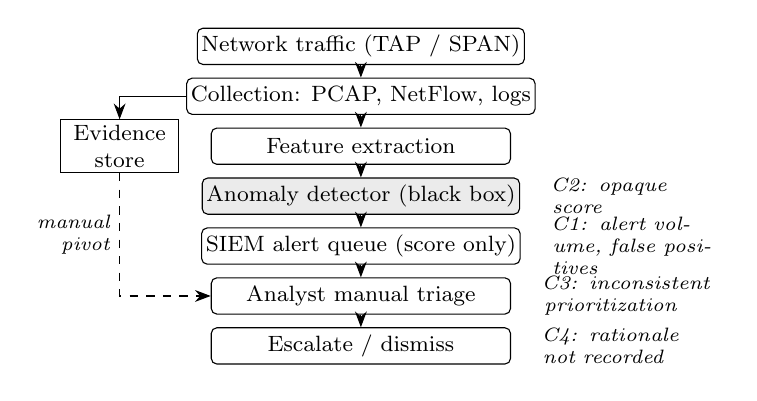
\begin{tikzpicture}[
  node distance=1.6mm,
  box/.style={draw, rounded corners=2pt, align=center, font=\footnotesize, minimum width=38mm, minimum height=4.6mm, inner sep=1.5pt},
  store/.style={draw, align=center, font=\footnotesize, minimum width=15mm, inner sep=2pt},
  tag/.style={align=left, font=\scriptsize\itshape, text width=21mm},
  arr/.style={-{Stealth[length=2mm]}}]
\node[box] (net) {Network traffic (TAP / SPAN)};
\node[box, below=of net] (col) {Collection: PCAP, NetFlow, logs};
\node[box, below=of col] (fe) {Feature extraction};
\node[box, below=of fe, fill=black!8] (det) {Anomaly detector (black box)};
\node[box, below=of det] (q) {SIEM alert queue (score only)};
\node[box, below=of q] (an) {Analyst manual triage};
\node[box, below=of an] (dec) {Escalate / dismiss};
\node[store, left=4mm of fe] (ev) {Evidence\\ store};
\draw[arr] (net) -- (col);
\draw[arr] (col) -- (fe);
\draw[arr] (fe) -- (det);
\draw[arr] (det) -- (q);
\draw[arr] (q) -- (an);
\draw[arr] (an) -- (dec);
\draw[arr] (col.west) -| (ev.north);
\draw[arr, dashed] (ev.south) |- node[pos=0.25, left, font=\scriptsize\itshape, align=right]{manual\\ pivot} (an.west);
\node[tag, right=3mm of det] (c2) {C2: opaque score};
\node[tag, right=3mm of q]   (c1) {C1: alert volume, false positives};
\node[tag, right=3mm of an]  (c3) {C3: inconsistent prioritization};
\node[tag, right=3mm of dec] (c4) {C4: rationale not recorded};
\end{tikzpicture}
\caption{Typical architecture of anomaly-detection-assisted forensic triage. The shaded stage is opaque to the analyst; tags C1--C4 mark the challenges discussed in Section~\ref{sec:challenges}.}
\label{fig:current}
\end{figure}

\subsection{Current Challenges in Digital Forensic Triage}
\label{sec:challenges}
The first challenge is alert volume (C1). Anomaly detectors flag anything unusual, and much unusual traffic is benign. Security operations analysts report that most of the alarms they receive are false positives and that the volume leads to fatigue and missed incidents \cite{alahmadi}; many alerts are also low-level and arrive without context \cite{cysider,gridsoc}. The second is the opacity of the score itself (C2). A score shows \emph{that} a flow is unusual but not \emph{why}, so the analyst must work out whether a rare port, a packet burst, or a large outbound transfer was responsible. Sommer and Paxson identified this semantic gap between a detector's output and its operational meaning as a central obstacle to deploying anomaly detection \cite{sommer}.

Without a stated reason behind each score, analysts fall back on individual experience to rank alerts, and prioritization becomes inconsistent (C3). Two analysts may triage the same alert differently, and neither decision is easy to review or reproduce. Accountability suffers as a result (C4). Forensic practice requires that the steps leading to a conclusion are documented and repeatable \cite{nist}. A decision based on an unexplained score, with the reasoning unrecorded, is hard to justify later in a report or in court, and the score itself is not evidence unless it is linked to preserved data. Underlying all four problems is the reliability of the models themselves (C5). Detectors are usually developed on lab benchmarks that contain labelling errors and artifacts \cite{engelen}, they can score well while relying on shortcut features that do not carry over to real networks \cite{trustee,arp}, and their accuracy can degrade without visible signs as traffic drifts.

\subsection{The Need for Explainable Anomaly Detection in Digital Forensic Triage}
Explainable AI addresses C2 directly: methods such as SHAP attribute a model's output to the input features that produced it \cite{shap}. Explanations alone, however, do not solve triage. Per-event attributions are technical, may change when the model or its reference data changes \cite{warnecke}, and can be manipulated \cite{fooling}. In our prior work on DER networks, SHAP attributions and the model's decision rules agreed only moderately (44.6\% average consistency) \cite{excyder}. Attributions also describe a single alert without saying what to do with it, so C1 and C3 remain. Rules give consistent guidance, but a rule set that only approximates the detector can misrepresent it, and neither approach leaves the record that C4 requires. Security operations for critical infrastructure likewise call for contributing factors or decision rules rather than opaque scores \cite{gridsoc}.

Forensic triage therefore needs an explainable anomaly-detection framework that satisfies five requirements, which the rest of this paper refers to. Explanations must be \emph{faithful} to what the detector actually computed (R1) and \emph{stable}, so that similar events receive similar explanations regardless of arbitrary configuration choices (R2). They must be \emph{actionable}, turning into concise and consistent priority decisions (R3), and every decision must be \emph{auditable}, meaning it can be reconstructed from preserved inputs (R4). Finally, the framework must keep the \emph{investigator in the loop}, supporting rather than replacing human judgement and making its own uncertainty visible (R5).

% ---------------------------------------------------------------------------
\begin{figure*}[t]
\centering
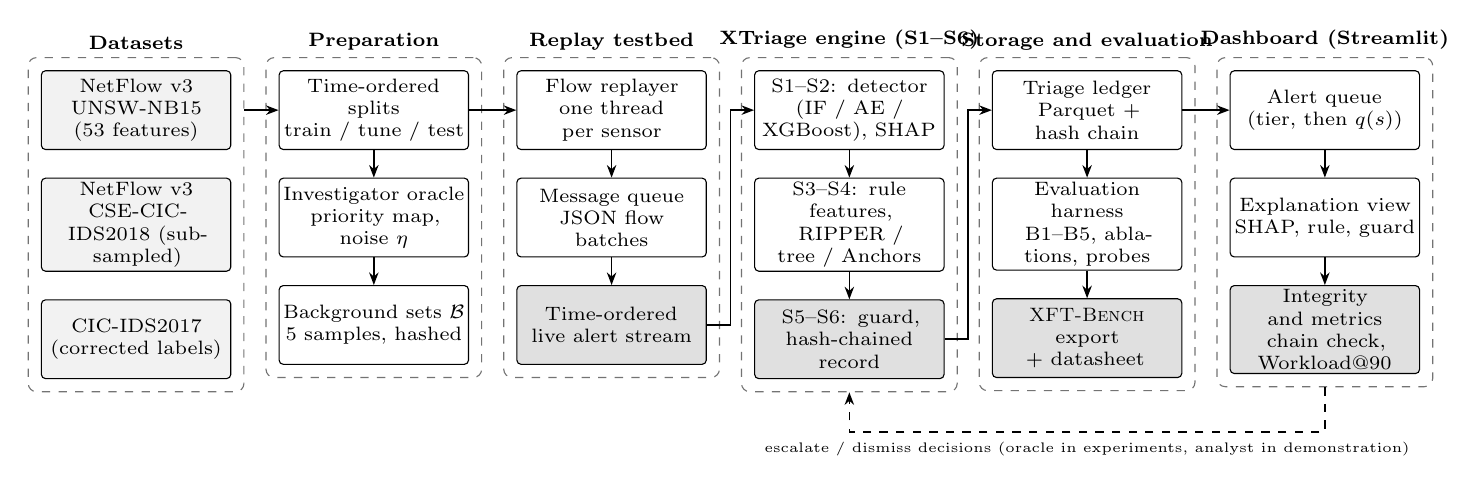
\begin{tikzpicture}[
  font=\scriptsize,
  box/.style={draw, rounded corners=1.5pt, align=center, text width=23mm, minimum height=10mm, inner sep=1.5pt, fill=white},
  data/.style={box, fill=black!5},
  hot/.style={box, fill=black!12},
  panel/.style={draw=black!55, dashed, rounded corners=3pt, inner sep=1.6mm},
  ptitle/.style={font=\scriptsize\bfseries, inner sep=1pt},
  arr/.style={-{Stealth[length=1.6mm]}, semithick},
  fb/.style={-{Stealth[length=1.6mm]}, semithick, dashed}]
% Datasets
\node[data] (d1) {NetFlow v3 UNSW-NB15\\(53 features)};
\node[data, below=3.5mm of d1] (d2) {NetFlow v3 CSE-CIC-\\IDS2018 (subsampled)};
\node[data, below=3.5mm of d2] (d3) {CIC-IDS2017\\(corrected labels)};
% Preparation
\node[box, right=6mm of d1] (split) {Time-ordered splits\\train / tune / test};
\node[box, below=3.5mm of split] (oracle) {Investigator oracle\\priority map, noise $\eta$};
\node[box, below=3.5mm of oracle] (bgs) {Background sets $\mathcal{B}$\\5 samples, hashed};
% Replay testbed
\node[box, right=6mm of split] (replay) {Flow replayer\\one thread per sensor};
\node[box, below=3.5mm of replay] (queue) {Message queue\\JSON flow batches};
\node[hot, below=3.5mm of queue] (stream) {Time-ordered\\live alert stream};
% Engine
\node[box, right=6mm of replay] (e1) {S1--S2: detector\\(IF / AE / XGBoost), SHAP};
\node[box, below=3.5mm of e1] (e2) {S3--S4: rule features,\\RIPPER / tree / Anchors};
\node[hot, below=3.5mm of e2] (e3) {S5--S6: guard,\\hash-chained record};
% Storage and evaluation
\node[box, right=6mm of e1] (ledger) {Triage ledger\\Parquet + hash chain};
\node[box, below=3.5mm of ledger] (harness) {Evaluation harness\\B1--B5, ablations, probes};
\node[hot, below=3.5mm of harness] (bench) {\textsc{XFT-Bench} export\\+ datasheet};
% Dashboard
\node[box, right=6mm of ledger] (v1) {Alert queue\\(tier, then $q(s)$)};
\node[box, below=3.5mm of v1] (v2) {Explanation view\\SHAP, rule, guard};
\node[hot, below=3.5mm of v2] (v3) {Integrity and metrics\\chain check, Workload@90};
% panels and titles
\node[panel, fit=(d1)(d3)] (P1) {};
\node[panel, fit=(split)(bgs)] (P2) {};
\node[panel, fit=(replay)(stream)] (P3) {};
\node[panel, fit=(e1)(e3)] (P4) {};
\node[panel, fit=(ledger)(bench)] (P5) {};
\node[panel, fit=(v1)(v3)] (P6) {};
\node[ptitle, above=0.5mm of P1.north] {Datasets};
\node[ptitle, above=0.5mm of P2.north] {Preparation};
\node[ptitle, above=0.5mm of P3.north] {Replay testbed};
\node[ptitle, above=0.5mm of P4.north] {\textsc{XTriage} engine (S1--S6)};
\node[ptitle, above=0.5mm of P5.north] {Storage and evaluation};
\node[ptitle, above=0.5mm of P6.north] {Dashboard (Streamlit)};
% flows between panels
\draw[arr] (P1.east |- split.west) -- (split.west);
\draw[arr] (split) -- (oracle);
\draw[arr] (oracle) -- (bgs);
\draw[arr] (split.east) -- (replay.west);
\draw[arr] (replay) -- (queue);
\draw[arr] (queue) -- (stream);
\draw[arr] (stream.east) -- ++(3mm,0) |- (e1.west);
\draw[arr] (e1) -- (e2);
\draw[arr] (e2) -- (e3);
\draw[arr] (e3.east) -- ++(3mm,0) |- (ledger.west);
\draw[arr] (ledger) -- (harness);
\draw[arr] (harness) -- (bench);
\draw[arr] (ledger.east) -- (v1.west);
\draw[arr] (v1) -- (v2);
\draw[arr] (v2) -- (v3);
% decision feedback
\coordinate (yb) at ($(P4.south)+(0,-5mm)$);
\draw[fb] (P6.south) -- (P6.south |- yb) -- node[below, font=\tiny]{escalate / dismiss decisions (oracle in experiments, analyst in demonstration)} (P4.south |- yb) -- (P4.south);
\end{tikzpicture}
\caption{Overview of the \textsc{XTriage} methodology. Public flow datasets are prepared into time-ordered splits, background sets, and oracle priorities; replayed through emulated sensors; and processed by the engine stages S1--S6 described in this section. Every decision is written to a hash-chained ledger that feeds the evaluation harness, the released benchmark, and a Streamlit dashboard. The dashed arrow returns escalate or dismiss decisions to the engine, supplied by the oracle during experiments and by an investigator in practice.}
\label{fig:pipeline}
\end{figure*}

\section{Related Work}
\label{sec:related}

Anomaly-based network intrusion detection learns a model of normal traffic and scores deviations from it, using isolation forests \cite{iforest} or autoencoder ensembles such as Kitsune \cite{kitsune}. Supervised gradient-boosted trees \cite{xgboost} usually achieve higher accuracy on labelled benchmarks, but they cannot recognize attack classes absent from their training data, which is precisely the case that anomaly detection exists to cover. How such models are evaluated matters as much as how they are built. Arp et al. \cite{arp} catalogued recurring pitfalls in security machine learning, including data snooping, spurious correlations, and unsuitable baselines, and Sarhan et al. \cite{sarhan} proposed a common NetFlow feature set so that results can be compared across datasets.

Because these detectors are opaque, much recent work has turned to post-hoc explanation. SHAP \cite{shap} assigns each feature an additive contribution based on Shapley values, and TreeSHAP computes these contributions exactly for tree ensembles \cite{treeshap}; LIME \cite{lime} instead fits a local linear surrogate around each prediction. Wang et al. \cite{wang} used SHAP to explain intrusion-detection decisions both for individual events and for the model as a whole, and Hermosilla et al. \cite{hermosilla} compared SHAP and LIME specifically for forensic intrusion analysis. Whether these explanations can be trusted is less settled. Warnecke et al. \cite{warnecke} found large differences between explanation methods in descriptive accuracy and stability, and Kalakoti et al. \cite{kalakoti} reached a similar conclusion on real SOC alerts. Maseno et al. \cite{maseno} showed on UNSW-NB15 that the most accurate detectors do not produce the most stable SHAP explanations across retraining, and Slack et al. \cite{fooling} demonstrated that local explanations can be made deliberately misleading. Closest to our goal, Gombar \cite{gombar} moved from detection toward triage by ranking flows with a priority score that combines classifier confidence, SHAP explanation strength, and attack severity.

A parallel line of work expresses model behaviour as rules rather than attributions. RIPPER \cite{ripper} learns compact rule lists that people can read directly, and Anchors \cite{anchors} produces high-precision rules that explain individual predictions. In network security, Trustee \cite{trustee} approximated black-box models with decision trees, measured how faithfully the trees reproduced the original models, and used them to expose shortcut learning in popular datasets, while Adewole et al. \cite{adewole} used rule induction to explain an IoT intrusion-detection system. Rudin \cite{rudin} takes the argument further, contending that high-stakes settings should use models that are interpretable by design rather than explained after the fact.

Our own prior work has combined these two strands for security operations in distributed energy resource (DER) networks. CySIDER \cite{cysider} attached decision-path explanations to edge anomaly alerts and correlated them with a knowledge graph. ExCyDER \cite{excyder} scored how well each alert's SHAP attributions agreed with its decision rules and marked low-scoring alerts as unverified. CyTReX \cite{cytrex} merged SHAP values, surrogate rules, and threat intelligence into an evidence packet from which a large language model ranked threat hypotheses, and found that a closed-set classifier pushes unseen attacks toward known classes. The grid SOC architecture in \cite{gridsoc} places explainability and human-governed escalation at the core of security operations. These studies, however, rely on supervised detectors trained on DNP3 traffic, and they use SHAP and rules only to check or describe individual alerts.

Table~\ref{tab:compare} summarizes this landscape. Explanation stability has been audited \cite{maseno,warnecke} and SHAP has been used to rank alerts \cite{gombar}, but separately and only for supervised classifiers; where attribution and rules are combined \cite{excyder,cytrex}, each serves only to check the other on individual alerts. To our knowledge, no prior work \emph{learns} triage rules from the explanations themselves, measures the effect on investigator workload together with rule fidelity and explanation stability on the same alerts, or releases the explanations as a benchmark so that these properties can be compared across studies. These three gaps define the contribution of this work.

\begin{table}[t]
\centering
\caption{Comparison With Representative Prior Work ($\circ$ = Partial)}
\label{tab:compare}
\setlength{\tabcolsep}{3pt}
\footnotesize
\begin{tabular}{@{}lccccc@{}}
\toprule
     & Local &       & Stability & Triage & Audit\\
Work & attr. & Rules & eval.     & metric & record\\
\midrule
Wang et al. \cite{wang}          & \checkmark & --         & --         & -- & -- \\
Warnecke et al. \cite{warnecke}  & \checkmark & --         & \checkmark & -- & -- \\
Trustee \cite{trustee}           & --         & \checkmark & --         & -- & -- \\
Adewole et al. \cite{adewole}    & --         & \checkmark & --         & -- & -- \\
Hermosilla et al. \cite{hermosilla} & \checkmark & --      & --         & -- & -- \\
Maseno et al. \cite{maseno}      & \checkmark & --         & \checkmark & -- & -- \\
Gombar \cite{gombar}             & \checkmark & --         & --         & $\circ$ & -- \\
ExCyDER \cite{excyder}          & \checkmark & \checkmark & $\circ$    & -- & -- \\
CyTReX \cite{cytrex}            & \checkmark & \checkmark & --         & $\circ$ & $\circ$ \\
This work                        & \checkmark & \checkmark & \checkmark & \checkmark & \checkmark \\
\bottomrule
\end{tabular}
\end{table}

% ---------------------------------------------------------------------------
\section{Methodology}
\label{sec:method}

The proposed framework, \textsc{XTriage}, adds explanation, rule induction, a consistency check, and record keeping to the architecture in Fig.~\ref{fig:current}. Fig.~\ref{fig:pipeline} gives an end-to-end view of the methodology. Public flow datasets are prepared into time-ordered splits, background sets, and oracle priorities, then replayed as live streams through the engine stages S1--S6 described below. Every decision is stored in a hash-chained ledger, from which the evaluation harness, the released benchmark, and the investigator dashboard are all served. Each flow is represented as a feature vector $\mathbf{x}\in\mathbb{R}^d$. Identifiers such as IP addresses, timestamps, and flow IDs are kept in the evidence record but excluded from the model input, so the model cannot learn shortcuts from them.

\subsection{S1: Anomaly Detection}
The primary detector is an isolation forest \cite{iforest} trained only on benign flows from an early time window. It never sees attack labels, so it can still flag attack types that did not appear in training, a case in which closed-set classifiers fail \cite{cytrex}. Its score $s=f(\mathbf{x})$ is converted to a percentile $q(s)\in[0,1]$ relative to held-out benign traffic. To check that findings do not depend on one model, we repeat the experiments with an autoencoder (reconstruction error) and with a supervised XGBoost classifier \cite{xgboost}, which serves as an upper-bound reference.

\subsection{S2: Event-Level Attribution (R1)}
For every alert ($q(s)\geq\theta$), SHAP splits the score into one contribution per feature,
\begin{equation}
f(\mathbf{x})=\phi_0+\textstyle\sum_{j=1}^{d}\phi_j(\mathbf{x}),
\end{equation}
where $\phi_0$ is the expected score over a benign background set $\mathcal{B}$. Tree models use exact TreeSHAP \cite{treeshap}; the autoencoder uses KernelSHAP. LIME \cite{lime} is included as a comparison method. Because SHAP values depend on $\mathcal{B}$, the hash of the background set is stored with every decision. The analyst sees the top-$k$ features ranked by contribution, together with the sign of each contribution; we denote this set $T_k(\mathbf{x})$.

\subsection{S3: SHAP-Augmented Representation}
Raw SHAP vectors are too detailed to drive consistent decisions, and rules learned only from raw features can capture patterns the detector does not actually use. We therefore combine three kinds of information in one representation:
\begin{equation}
\mathbf{z}(\mathbf{x})=\big[\,\mathrm{disc}(\mathbf{x}),\;\pi_1(\mathbf{x}),\dots,\pi_d(\mathbf{x}),\;\mathrm{band}(q(s))\,\big].
\end{equation}
Here $\mathrm{disc}(\cdot)$ assigns each feature to a quantile bin, and $\mathrm{band}(\cdot)$ maps the score percentile to low, medium, or high. Each SHAP predicate $\pi_j(\mathbf{x})=\mathbb{1}[\,j\in T_k(\mathbf{x})\wedge\phi_j(\mathbf{x})>0\,]$ is true when feature $j$ was among the main reasons the flow looked anomalous. Rules can therefore combine \emph{what the traffic looked like} with \emph{why the detector reacted}:
\begin{quote}\footnotesize
IF band$=$high AND $\pi_{\text{dst\_port}}$ AND out\_bytes$\,\in\,$Q5 THEN P1.
\end{quote}

\subsection{S4: Rule Induction (R3)}
Each event receives one of three priorities $p\in\{\text{P1},\text{P2},\text{P3}\}$: escalate, review, or dismiss. RIPPER \cite{ripper} learns an ordered rule list $R(\mathbf{z})$ from investigator decisions that have been checked against evidence. The framework is therefore \emph{semi-supervised}: the detector never sees labels, but the triage rules are learned from confirmed decisions, as in an operational SOC. Rules are limited to at most four conditions so that they stay readable. We compare RIPPER with two alternatives: a depth-limited decision-tree surrogate in the style of Trustee \cite{trustee}, and Anchors \cite{anchors}, which explains one event at a time. Every rule is versioned and stored with its support and precision on the training data.

\subsection{S5: Disagreement Guard (R5)}
Rules simplify the detector, and the simplification can be wrong. Extending the per-alert verification of ExCyDER \cite{excyder} from explanations to decisions, the guard marks a case as \emph{contested} and sends it for manual review when (i)~only RIPPER's default (catch-all) rule fires, or (ii)~the rule's priority conflicts with the score. Examples of conflict are a P3 (dismiss) rule firing on a flow with $q(s)\geq 0.99$, or a P1 (escalate) rule firing on a flow in the low score band. Within each tier, alerts are ranked by $q(s)$, and rule errors are shown to the analyst rather than hidden.

\subsection{S6: Forensic Triage Record (R4)}
Each decision is appended to a record $r_i$. The record holds the flow identifiers and features; a hash reference to the source capture; $s$, $q(s)$, and $\boldsymbol{\phi}$; the hash of $\mathcal{B}$; the rule that fired; the model and rule-set versions; the guard status; a timestamp; and the investigator's response. Records are chained by computing $h_i=\mathrm{SHA256}(h_{i-1}\,\|\,r_i)$, so tampering with any earlier record is detectable, and every decision can be replayed exactly from its stored inputs \cite{nist}.

\subsection{Feedback and Implementation}
Investigator responses update the rules only after they have been confirmed against preserved evidence. Rules are re-learned on a fixed schedule rather than continuously, and each new version must pass a frozen test set before release. The framework will be implemented in Python with scikit-learn, the \texttt{shap} library, and an open-source RIPPER implementation, and the records will be stored as Parquet files.

% ---------------------------------------------------------------------------
\section{Evaluation Setup}
\label{sec:eval}

\subsection{Experimental Testbed}
Fig.~\ref{fig:testbed} shows the testbed. Rather than scoring a static test file, the testbed replays each time-ordered test window as a live stream. A set of Python worker threads, each emulating one network sensor, reads flow records in timestamp order and publishes them to a message queue in fixed-size JSON batches, the same edge-to-analytics pattern used in our earlier SOC prototypes \cite{cysider,excyder}. The \textsc{XTriage} engine consumes the batches, so alerts reach the analyst in the order they would arrive in practice, and the latency of each stage (scoring, attribution, rule evaluation, guard check, and record write) can be measured. Every decision is appended to a triage ledger stored as Parquet files with the hash chain of Section~\ref{sec:method}. An evaluation harness reads the ledger to run the baselines, ablations, and limitation probes over five seeds and to export \textsc{XFT-Bench}.

The analyst dashboard is built in Streamlit, which runs in the same Python environment as the engine and matches our earlier prototypes \cite{cysider,cytrex}. It provides three views: an alert queue ordered by priority tier and score percentile; an explanation view that shows each alert's SHAP attributions, the rule that fired, and the guard status; and an integrity and metrics view that re-verifies the hash chain and plots workload and stability metrics as the stream progresses. The dashboard also accepts manual escalate or dismiss decisions, which are written to the ledger in the same way as oracle decisions. In the quantitative experiments the oracle supplies all decisions and every reported number comes from the harness; the dashboard serves to demonstrate the investigator workflow and to inspect individual cases.

\begin{figure*}[t]
\centering
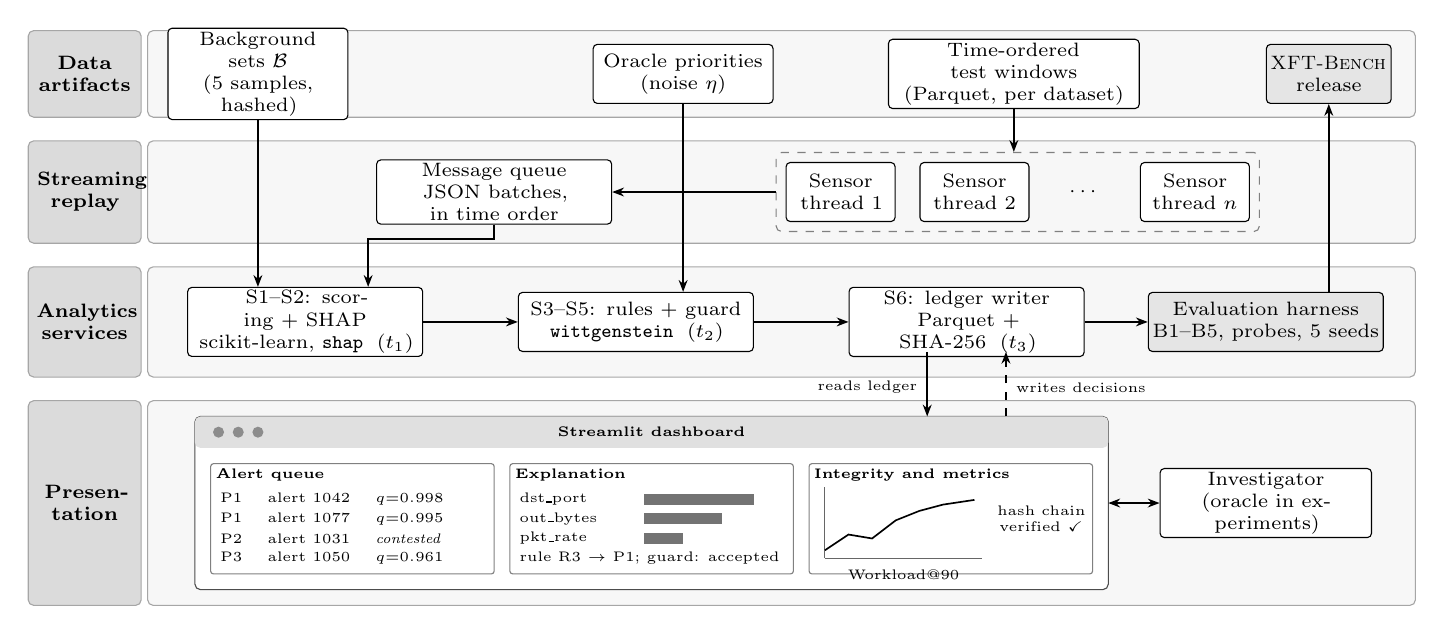
\begin{tikzpicture}[x=1mm, y=1mm,
  font=\scriptsize,
  lane/.style={draw=black!35, fill=black!3, rounded corners=2pt},
  lname/.style={draw=black!35, fill=black!14, rounded corners=2pt, align=center, font=\scriptsize\bfseries, text width=12mm},
  box/.style={draw, rounded corners=1.5pt, align=center, fill=white, minimum height=7.5mm, inner sep=1.2pt},
  hot/.style={box, fill=black!10},
  arr/.style={-{Stealth[length=1.5mm]}, semithick},
  fb/.style={-{Stealth[length=1.5mm]}, semithick, dashed},
  tile/.style={draw=black!50, fill=white, rounded corners=1pt},
  tt/.style={font=\tiny\bfseries, anchor=north west, inner sep=0.8pt},
  tx/.style={font=\tiny, anchor=west, inner sep=0.5pt}]
% ---- lanes
\draw[lane] (16,0) rectangle (177,-11);
\draw[lane] (16,-14) rectangle (177,-27);
\draw[lane] (16,-30) rectangle (177,-44);
\draw[lane] (16,-47) rectangle (177,-73);
\node[lname, minimum height=11mm] at (8,-5.5) {Data\\artifacts};
\node[lname, minimum height=13mm] at (8,-20.5) {Streaming\\replay};
\node[lname, minimum height=14mm] at (8,-37) {Analytics\\services};
\node[lname, minimum height=26mm] at (8,-60) {Presen-\\tation};
% ---- data artifacts
\node[box, text width=22mm] (bg) at (30,-5.5) {Background sets $\mathcal{B}$\\(5 samples, hashed)};
\node[box, text width=22mm] (orc) at (84,-5.5) {Oracle priorities\\(noise $\eta$)};
\node[box, text width=31mm] (split) at (126,-5.5) {Time-ordered test windows\\(Parquet, per dataset)};
\node[hot, text width=15mm] (bench) at (166,-5.5) {\textsc{XFT-Bench}\\release};
% ---- streaming replay
\node[box, text width=29mm] (mq) at (60,-20.5) {Message queue\\JSON batches, in time order};
\node[box, text width=13mm] (s1) at (104,-20.5) {Sensor\\thread 1};
\node[box, text width=13mm] (s2) at (121,-20.5) {Sensor\\thread 2};
\node at (135,-20.5) {$\cdots$};
\node[box, text width=13mm] (sn) at (149,-20.5) {Sensor\\thread $n$};
\node[draw=black!50, dashed, rounded corners=2pt, inner sep=1.2mm, fit=(s1)(sn)] (G) {};
% ---- analytics services
\node[box, text width=29mm] (e1) at (36,-37) {S1--S2: scoring + SHAP\\scikit-learn, \texttt{shap} \;($t_1$)};
\node[box, text width=29mm] (e2) at (78,-37) {S3--S5: rules + guard\\\texttt{wittgenstein} \;($t_2$)};
\node[box, text width=29mm] (e3) at (120,-37) {S6: ledger writer\\Parquet + SHA-256 \;($t_3$)};
\node[hot, text width=29mm] (har) at (158,-37) {Evaluation harness\\B1--B5, probes, 5 seeds};
% ---- presentation: dashboard mock-up
\draw[draw=black!70, fill=white, rounded corners=2pt] (22,-49) rectangle (138,-71);
\fill[black!12, rounded corners=2pt] (22,-49) rectangle (138,-53);
\foreach \cx in {25,27.5,30} \fill[black!45] (\cx,-51) circle (0.7);
\node[font=\tiny\bfseries] at (80,-51) {Streamlit dashboard};
\draw[tile] (24,-55) rectangle (60,-69);
\draw[tile] (62,-55) rectangle (98,-69);
\draw[tile] (100,-55) rectangle (136,-69);
\node[tt] at (24.3,-55.3) {Alert queue};
\node[tt] at (62.3,-55.3) {Explanation};
\node[tt] at (100.3,-55.3) {Integrity and metrics};
% queue rows
\node[tx] at (25,-59.5) {P1 \quad alert 1042 \quad $q{=}0.998$};
\node[tx] at (25,-62)   {P1 \quad alert 1077 \quad $q{=}0.995$};
\node[tx] at (25,-64.5) {P2 \quad alert 1031 \quad \emph{contested}};
\node[tx] at (25,-67)   {P3 \quad alert 1050 \quad $q{=}0.961$};
% SHAP bars
\node[tx] at (63,-59.5) {dst\_port};   \fill[black!55] (79,-60.2) rectangle (93,-58.8);
\node[tx] at (63,-62)   {out\_bytes};  \fill[black!55] (79,-62.7) rectangle (89,-61.3);
\node[tx] at (63,-64.5) {pkt\_rate};   \fill[black!55] (79,-65.2) rectangle (84,-63.8);
\node[tx] at (63,-67)   {rule R3 $\rightarrow$ P1; guard: accepted};
% metrics chart and chain check
\draw[black!60] (102,-67) -- (122,-67);
\draw[black!60] (102,-67) -- (102,-58);
\draw[semithick] (102,-66) -- (105,-64) -- (108,-64.5) -- (111,-62.2) -- (114,-61) -- (117,-60.2) -- (121,-59.6);
\node[font=\tiny, anchor=north] at (112,-67.2) {Workload@90};
\node[font=\tiny, align=center] at (129.5,-62) {hash chain\\verified \checkmark};
% investigator
\node[box, text width=26mm] (inv) at (158,-60) {Investigator\\(oracle in experiments)};
% ---- arrows
\draw[arr] (split.south) -- (split.south |- G.north);
\draw[arr] (G.west) -- (mq.east);
\draw[arr] (mq.south) -- ++(0,-1.8) -| ($(e1.north)+(8,0)$);
\draw[arr] (bg.south) -- (bg.south |- e1.north);
\draw[arr] (orc.south) -- (orc.south |- e2.north);
\draw[arr] (e1) -- (e2);
\draw[arr] (e2) -- (e3);
\draw[arr] (e3) -- (har);
\draw[arr] (har.north -| bench) -- (bench.south);
\draw[arr] (115,-40.8) -- node[pos=0.55, left, font=\tiny]{reads ledger} (115,-49);
\draw[fb] (125,-49) -- node[pos=0.45, right, font=\tiny]{writes decisions} (125,-40.8);
\draw[{Stealth[length=1.5mm]}-{Stealth[length=1.5mm]}, semithick] (138,-60) -- (inv.west);
\end{tikzpicture}
\caption{Experimental testbed, organized by layer. Time-ordered test windows are replayed by $n$ sensor threads into a message queue. The analytics services score, explain, and triage each alert and append it to the hash-chained ledger, recording the per-stage latencies $t_1$--$t_3$; the evaluation harness reads the ledger to compute all reported metrics and export \textsc{XFT-Bench}. The Streamlit dashboard (sketched) reads the same ledger, and decisions entered there are written back to it. In the quantitative experiments the oracle supplies every decision.}
\label{fig:testbed}
\end{figure*}

\subsection{Datasets}
Evaluation uses the NetFlow v3 versions of UNSW-NB15 and CSE-CIC-IDS2018 \cite{nfv3,sarhan,unsw}. Both describe flows with the same 53 features, including flow start and end times, so a model trained on one can be tested on the other and the data can be split by time. CIC-IDS2017 \cite{cicids}, with the corrections from \cite{engelen}, is used for comparison with prior work. The full CIC-IDS2018 data (about 19M flows) is subsampled by time window, and the slower methods (KernelSHAP, LIME, Anchors) run on a stratified sample of alerts. All splits are by time: the detector and the background set come from the earliest window, rule induction and tuning use the middle window, and testing uses the latest. This follows \cite{arp} and prevents leakage from later traffic.

\subsection{Investigator Oracle}
Because real analysts' decisions are not available for these corpora, a documented \emph{oracle} stands in for them. The oracle maps each dataset's own attack classes to priorities by likely impact: code execution and persistence (e.g., Exploits, Backdoor, and Shellcode in UNSW-NB15; Infilteration and Bot in CIC-IDS2018) to P1; reconnaissance, fuzzing, brute force, and DoS to P2; and benign to P3. It also flips a fraction $\eta\in\{0,0.1,0.2,0.3\}$ of them at random to simulate analyst error.

\subsection{Released Benchmark: \textsc{XFT-Bench}}
Running the framework on these corpora produces an explained-triage dataset, which we will release. For every test flow it includes the score, the SHAP values (computed with five background samples and three detector seeds so that others can study stability), the rule that fired, the guard status, the oracle priority, and the ground-truth label. It also contains the splits, rule sets, a datasheet, and regeneration scripts, subject to the upstream licences.

\subsection{Research Questions and Metrics}
Table~\ref{tab:rq} maps each research question to its requirement and metrics. We hypothesize the following. For RQ1, \textsc{XTriage} finds as many P1 events as score-only ranking while requiring fewer alerts to be reviewed. For RQ2, attributions are stable for clear-cut attacks but unstable for alerts that score close to the threshold. For RQ3, rules learned on $\mathbf{z}$ match the detector more closely and are more compact than rules learned on raw features, at equal accuracy.

\begin{table}[t]
\centering
\caption{Research Questions, Requirements, and Metrics}
\label{tab:rq}
\footnotesize
\setlength{\tabcolsep}{3pt}
\begin{tabular}{@{}p{22mm}p{8.5mm}p{53mm}@{}}
\toprule
Question & Req. & Metrics\\
\midrule
RQ1 Triage effectiveness & R3 & AUROC, AUPRC; P1 Recall@$b$ under alert budget $b$; Workload@90 (alerts reviewed to find 90\% of P1 events); NDCG\\
RQ2 Explanation reliability & R1, R2 & Top-$k$ Jaccard and Kendall's $\tau$ across backgrounds and seeds; deletion-curve faithfulness\\
RQ3 Rule quality & R3 & Fidelity to the detector; macro-F1 against the oracle; coverage; number of rules; mean rule length\\
RQ4 Limitations & R1--R5 & Change in the metrics above under each probe\\
RQ5 Accountability & R4, R5 & Replay success rate; bytes per record; contested-case rate; per-stage latency\\
\bottomrule
\end{tabular}
\end{table}

\subsection{Baselines and Ablations}
\textsc{XTriage} is compared with five baselines. The simplest (B1) ranks alerts by isolation-forest score alone, while B2 pairs a supervised XGBoost classifier with SHAP but learns no rules. B3 learns RIPPER rules on raw features only, representing the interpretable-by-design position of \cite{rudin}; B4 replaces the rule list with a decision-tree surrogate \cite{trustee}; and B5 substitutes LIME for SHAP. Ablations then remove the SHAP predicates, the score band, and the guard one at a time to isolate each component's contribution.

\subsection{Limitation Probes}
RQ4 deliberately looks for conditions under which explainable triage fails. To test sensitivity to the reference data, we vary the size, time window, and traffic mix of the background set $\mathcal{B}$ and measure how much the attributions and fired rules change. To expose shortcut learning, we remove port and TTL-like features and check whether performance and explanations collapse together, as reported for popular benchmarks \cite{engelen,trustee}. For distribution shift, we train on one corpus and test on the other and compare early with late time windows. A benign baseline from one network is expected to transfer poorly, so this probe characterizes \emph{how} rules and explanations fail rather than whether they fail.

Three further probes target the triage layer directly. A feature-space evasion test perturbs attacker-controllable features such as padding, timing, and port choice within protocol limits and compares how often rules stop firing with how much the score changes; it measures sensitivity in feature space and does not generate real attack traffic. A rule-infidelity test locates regions where rules and detector disagree and checks whether the guard catches them. Finally, sweeping the oracle noise rate $\eta$ shows how quickly rule quality degrades when investigator feedback is unreliable.

\subsection{Protocol and Threats to Validity}
Each configuration is run with five seeds (mean $\pm$ s.d.), compared with the Wilcoxon signed-rank test at $\alpha=0.05$, and preprocessed using training data only. Threats to validity: the oracle only approximates human judgement, lab corpora may not reflect production networks \cite{sommer}, and NetFlow lacks payloads, which limits what any explanation can reveal.

\begin{thebibliography}{00}
\bibitem{nist} K. Kent, S. Chevalier, T. Grance, and H. Dang, ``Guide to integrating forensic techniques into incident response,'' NIST SP 800-86, 2006.
\bibitem{iforest} F. T. Liu, K. M. Ting, and Z.-H. Zhou, ``Isolation forest,'' in \emph{Proc. IEEE ICDM}, 2008, pp. 413--422.
\bibitem{kitsune} Y. Mirsky, T. Doitshman, Y. Elovici, and A. Shabtai, ``Kitsune: An ensemble of autoencoders for online network intrusion detection,'' in \emph{Proc. NDSS}, 2018.
\bibitem{alahmadi} B. A. Alahmadi, L. Axon, and I. Martinovic, ``99\% false positives: A qualitative study of SOC analysts' perspectives on security alarms,'' in \emph{Proc. USENIX Security}, 2022.
\bibitem{sommer} R. Sommer and V. Paxson, ``Outside the closed world: On using machine learning for network intrusion detection,'' in \emph{Proc. IEEE S\&P}, 2010, pp. 305--316.
\bibitem{engelen} G. Engelen, V. Rimmer, and W. Joosen, ``Troubleshooting an intrusion detection dataset: The CICIDS2017 case study,'' in \emph{Proc. IEEE SPW}, 2021, pp. 7--12.
\bibitem{trustee} A. S. Jacobs \emph{et al.}, ``AI/ML for network security: The emperor has no clothes,'' in \emph{Proc. ACM CCS}, 2022.
\bibitem{arp} D. Arp \emph{et al.}, ``Dos and don'ts of machine learning in computer security,'' in \emph{Proc. USENIX Security}, 2022.
\bibitem{shap} S. M. Lundberg and S.-I. Lee, ``A unified approach to interpreting model predictions,'' in \emph{Adv. Neural Inf. Process. Syst.}, vol. 30, 2017.
\bibitem{warnecke} A. Warnecke, D. Arp, C. Wressnegger, and K. Rieck, ``Evaluating explanation methods for deep learning in security,'' in \emph{Proc. IEEE EuroS\&P}, 2020, pp. 158--174.
\bibitem{fooling} D. Slack, S. Hilgard, E. Jia, S. Singh, and H. Lakkaraju, ``Fooling LIME and SHAP: Adversarial attacks on post hoc explanation methods,'' in \emph{Proc. AAAI/ACM AIES}, 2020, pp. 180--186.
\bibitem{xgboost} T. Chen and C. Guestrin, ``XGBoost: A scalable tree boosting system,'' in \emph{Proc. ACM KDD}, 2016, pp. 785--794.
\bibitem{sarhan} M. Sarhan, S. Layeghy, and M. Portmann, ``Towards a standard feature set for network intrusion detection system datasets,'' \emph{Mobile Netw. Appl.}, vol. 27, pp. 357--370, 2022.
\bibitem{treeshap} S. M. Lundberg \emph{et al.}, ``From local explanations to global understanding with explainable AI for trees,'' \emph{Nat. Mach. Intell.}, vol. 2, pp. 56--67, 2020.
\bibitem{lime} M. T. Ribeiro, S. Singh, and C. Guestrin, ```Why should I trust you?': Explaining the predictions of any classifier,'' in \emph{Proc. ACM KDD}, 2016, pp. 1135--1144.
\bibitem{wang} M. Wang, K. Zheng, Y. Yang, and X. Wang, ``An explainable machine learning framework for intrusion detection systems,'' \emph{IEEE Access}, vol. 8, pp. 73127--73141, 2020.
\bibitem{hermosilla} P. Hermosilla, S. Berr\'ios, and H. Allende-Cid, ``Explainable AI for forensic analysis: A comparative study of SHAP and LIME in intrusion detection models,'' \emph{Appl. Sci.}, vol. 15, no. 13, Art. no. 7329, 2025.
\bibitem{ripper} W. W. Cohen, ``Fast effective rule induction,'' in \emph{Proc. ICML}, 1995, pp. 115--123.
\bibitem{anchors} M. T. Ribeiro, S. Singh, and C. Guestrin, ``Anchors: High-precision model-agnostic explanations,'' in \emph{Proc. AAAI}, 2018.
\bibitem{adewole} K. S. Adewole, A. Jacobsson, and P. Davidsson, ``Intrusion detection framework for Internet of Things with rule induction for model explanation,'' \emph{Sensors}, vol. 25, no. 6, Art. no. 1845, 2025.
\bibitem{rudin} C. Rudin, ``Stop explaining black box machine learning models for high stakes decisions and use interpretable models instead,'' \emph{Nat. Mach. Intell.}, vol. 1, pp. 206--215, 2019.
\bibitem{unsw} N. Moustafa and J. Slay, ``UNSW-NB15: A comprehensive data set for network intrusion detection systems,'' in \emph{Proc. MilCIS}, 2015.
\bibitem{cicids} I. Sharafaldin, A. H. Lashkari, and A. A. Ghorbani, ``Toward generating a new intrusion detection dataset and intrusion traffic characterization,'' in \emph{Proc. ICISSP}, 2018, pp. 108--116.
\bibitem{kalakoti} R. Kalakoti, R. Vaarandi, H. Bahsi, and S. N\~{o}mm, ``Evaluating explainable AI for deep learning-based network intrusion detection system alert classification,'' in \emph{Proc. ICISSP}, 2025.
\bibitem{maseno} E. M. Maseno, Y. Sun, and Z. Wang, ``Reliability auditing of explanations for machine-learning-based intrusion detection systems,'' \emph{J. Comput. Virol. Hacking Tech.}, vol. 22, Art. no. 80, 2026.
\bibitem{gombar} M. Gombar, ``From detection to triage: Explainable suspicious flow prioritization for multiclass intrusion detection using CSE-CIC-IDS2018,'' \emph{Electronics}, vol. 15, no. 12, Art. no. 2739, 2026.
\bibitem{nfv3} University of Queensland, ``NetFlow v3 datasets,'' [Online]. Available: https://staff.itee.uq.edu.au/marius/NIDS\_datasets/, accessed Oct. 2026.
\bibitem{gridsoc} D. Popoola, S. Bhattacharya, A. Hahn, and M. Govindarasu, ``AI-enabled security operations center (SOC) for modern power grids: Bridging the gap between the cybersecurity and grid operations,'' \emph{IEEE Power Energy Mag.}, pp. 57--69, Sep./Oct. 2026, doi: 10.1109/MPE.2026.3705348.
\bibitem{cysider} D. Popoola, S. Bhattacharya, and M. Govindarasu, ``CySIDER: Cybersecurity situational intelligence framework for DER networks,'' in \emph{Proc. Resilience Week (RWS)}, National Harbor, MD, USA, 2025, pp. 1--10, doi: 10.1109/RWS66711.2025.11304446.
\bibitem{excyder} D. Popoola, S. Bhattacharya, and M. Govindarasu, ``Self-verifying anomaly detection using explainable AI for cybersecurity of DER networks,'' in \emph{Proc. IEEE PES General Meeting (PESGM)}, 2026.
\bibitem{cytrex} D. Popoola, S. Bhattacharya, and M. Govindarasu, ``CyTReX: Explainable AI-based cybersecurity threat reasoning framework for DER networks,'' presented at \emph{Resilience Week (RWS)}, National Harbor, MD, USA, 2026, arXiv:2610.04286.
\end{thebibliography}

\end{document}
